\documentclass[12pt, letterpaper]{article}
\usepackage{listings}
\usepackage{color}
\usepackage{graphicx}
\usepackage{caption}
\usepackage{subcaption}
\usepackage[margin=1in]{geometry}
\usepackage[hidelinks]{hyperref}
\usepackage[backend=biber,style=numeric]{biblatex}
\addbibresource{citations.bib}
\graphicspath{{images/}}
\begin{document}

\begin{titlepage}
    \begin{center}
        \vspace*{1cm}
            
        \Huge
        \textbf{Interaction Design for Large Displays}
        
        \vspace{0.5cm}
        \LARGE
        An Analysis of Smart TV User Interfaces 
            
        \vspace{1.5cm}
            
        \textbf{Colter Roche}
            
        \vfill
          
        \Large
        Human Computer Interaction\\
        CEN4721\\
        \today
            
    \end{center}
\end{titlepage}

\newpage
\tableofcontents
\thispagestyle{empty}
\newpage
\section{Introduction}
Smart internet connected TVs and streaming devices are widely available and reasonably affordable for most people in 2021.  Almost 75\% of U.S. households
had at least one connected TV device in 2019, and the share of the market that is specifically Smart TVs is increasing every year\cite{leichtman_research_group_2019}.  With so many people consuming and searching for 
content in a large screen format, the interface design needs to be easy to use and effective for a wide variety of users and use cases.  

The four primary operating systems are Tizen OS from Samsung, WebOS from LG, tvOS from Apple, and Google TV/Android TV from Google.  These make up the largest share of the market, although 
Google TV is a relative latecomer, derived from Google's popular Android TV operating system\cite{alam_khusro_khan_2020}.  Android TVs from various brands are outside the scope of this report as each manufacturer tends to customize the design. Each brand and OS has
its own design language and standards, as well as a variety of input methods.  This report will cover each OS's interface design including software, hardware interface devices (remotes), and general consistency of experience 
across applications in the Smart TV's app ecosystem.  Interface design for specific 3rd party applications are outside the scope of this report, but 
issues surrounding inconsistencies with input systems and UI optimizations will be covered.
\begin{figure}[h]
    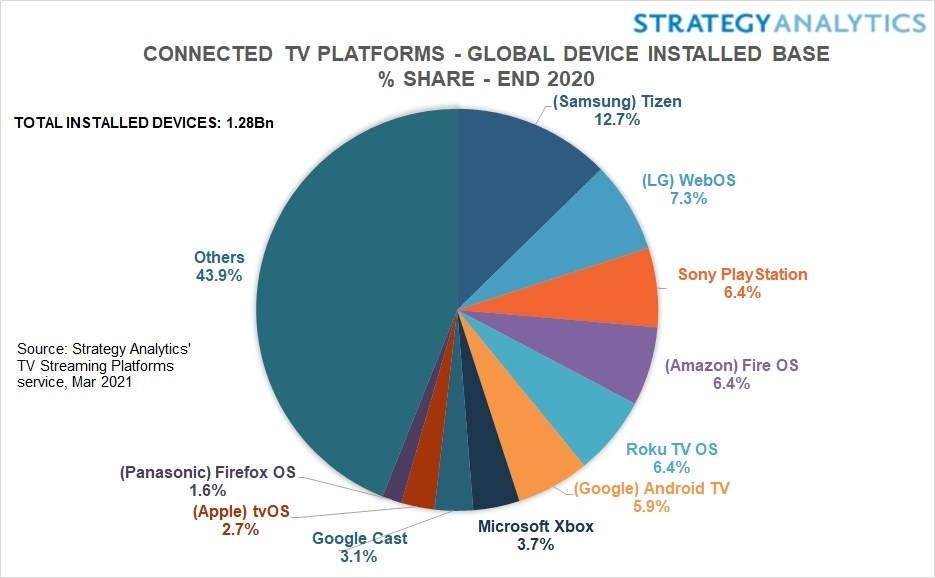
\includegraphics[width=\textwidth]{CTV_Platform_Global_IB_0321.jpg}
    \caption{Chart of connected TV OS platform percentages}
\end{figure}
TV is a "lean-back" form of media consumption, focused primarily on passively watching content rather than actively interacting with the device.  The main 
goal of the user interface is to allow the user to access the content they wish to view easily, provide useful information, and suggest more content options\cite{7774793}.  Older TV hardware tends to be low powered, limiting the options for animations 
and transitions in the graphical user interface (GUI), but more recent TVs and streaming devices are equipped with faster processors and more memory, allowing for more complex designs and a better user experience.  
One major issue that is especially prevalent in TV interface design is a tendency to pack unnecessary features and options into the interface, leading to bloat and cognitive overload.  With the vast amount of content available on the web,
users have many more options to choose from compared to traditional cable TV.  How these options are presented has a large impact on whether the viewer can easily find what they want to watch, or whether they lose patience or focus.  

This paper analyzes the pros and cons of the different interface designs that each OS uses, and contrasts the different approaches based on usability and user experience factors.  To gauge user experience, reviews of the interface for each OS were consulted, and 
user reviews from the product pages on Amazon and Newegg were also analyzed.  

\section{WebOS}
Originally created by Palm Inc. and then later open sourced by Hewlett Packard, WebOS is a Linux based OS built primarily for use with TVs and mobile devices and is currently managed by LG\cite{enwiki:1012760174}.
LG's design principles call for a simple to use interface with a focus on bright colors and fluid animations. WebOS is found almost exclusively on LG TVs and some appliances, and accounted for around 7\% of the smart TV market share in 2020\cite{strategy_analytics_2020}.  As of 2021, LG is ending
their exclusivity deal and WebOS will be available on other TV brands.  
\subsection{GUI}
WebOS's user interface consists of a smart home menu, an always available launcher, a preview area, and a system area. The various settings menus are clearly labeled and identified by a brightly colored icons.  WebOS uses a series of narrow blades arranged as a tabbed list along the bottom of the screen in the launcher menu,
featuring installed apps, input sources, and pinned TV channels.  Apps are sorted by relevance, with frequently used apps grouped nearer to the left side of the screen.  All UI elements are required to clearly indicate whether they are selected or not.  Buttons and select-able items are highlighted with a highly visible border when selected, 
and application cards in the launcher are larger and appear to be raised above the other cards in the menu when the user is hovering over them.  Nearly all UI transitions in WebOS use subtle animations to give a clear sense of movement.  Items bounce slightly when selected, and the close button for killing running 
applications briefly turns into a frowning face when clicked.  The use of these often whimsical animations increases the feelings of positive emotions and increases the user enjoyment when using the interface.  
\begin{figure}[h]
    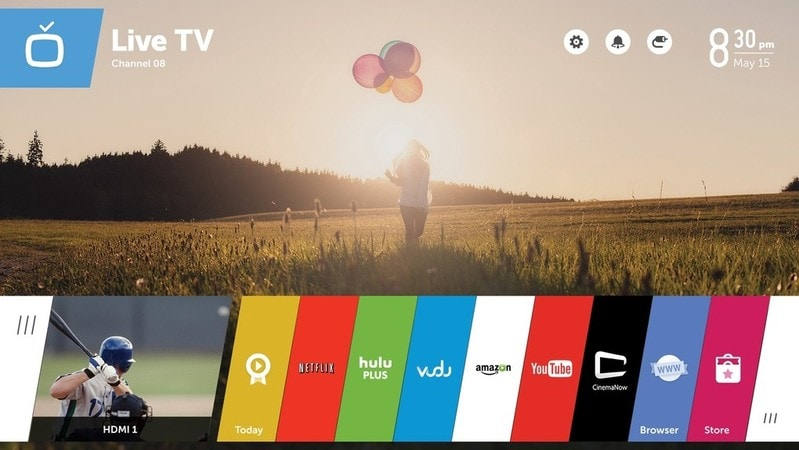
\includegraphics[width=\textwidth]{lg-webos.jpeg}
    \caption{The webOS Launcher blades.}
\end{figure}
\newpage
The launcher can be opened at any time and from within any app. Only the bottom edge of the screen is covered, 
allowing the user to see what is currently happening in the running app rather than completely obscuring the screen.  The launcher also displays previews of what other applications are currently displaying.  Unlike most other TV OSs, WebOs does not present the user with a long list of possible shows from installed applications 
on the main screen.  Instead, installed applications and input sources are listed unobtrusively in the launcher, reducing the cognitive overload from too many options at once. Application blades are consistently labelled, with either a white background with the service's name or a colored background for system applications. Hovering over or focusing on an application brings up 
a list of suggested shows or other content from that service, which can be easily selected. The launcher scrolls horizontally to the right, with less frequently used apps 
appearing further to the right.  Applications can also be uninstalled directly from the launcher, reducing the amount of time users need to spend searching through menus.

The LG Content Store serves as WebOS's content aggregation and search interface.  Movies, TV shows, and other applications can all be accessed from this system application. Selecting a show from the content store will bring up a list of streaming services installed that offer that program and will allow the user to smoothly switch to that program.
There is also a home dashboard that allows the user to control their smart home devices directly from the TV and view recommended content.  WebOS has a robust artificial intelligence powered recommendation system for arranging menus and suggesting content, lessening the amount of time users need to spend actively searching for shows. WebOS also supports streaming and accessing user content on external devices,
and includes that content in search results.
\begin{figure}
    \centering
    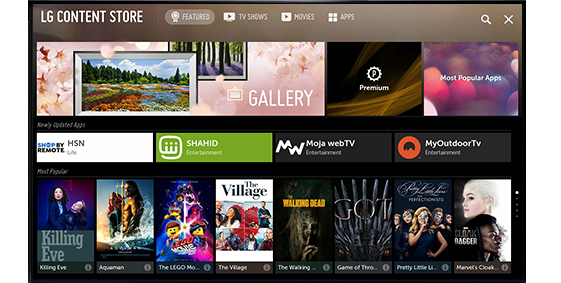
\includegraphics[width=0.7\textwidth]{main_visual_1_ch1.png}
    \caption{webOS's Content }
\end{figure}
\newpage
WebOS also has an animated virtual assistant named Bean Bird that helps walk the user through how to set up the different services on the TV when they first turn it on.  Short animations and scenes walk the user through the setup process, and Bean Bird praises or gently mocks the user depending on whether they set up all the features.  The agent's design is simplistic and the scenes are surprisingly fun to look 
at and engage with (See Figure \ref{Bean_Bird}).  According to WebOS's UX designer, LG saw a sharp increase in activations after Bean Bird was introduced.  The bird only appears during setup and updates, avoiding some of the annoyances of the ever-present Clippy in MS Windows 97.
\begin{figure}[h]
    \centering
    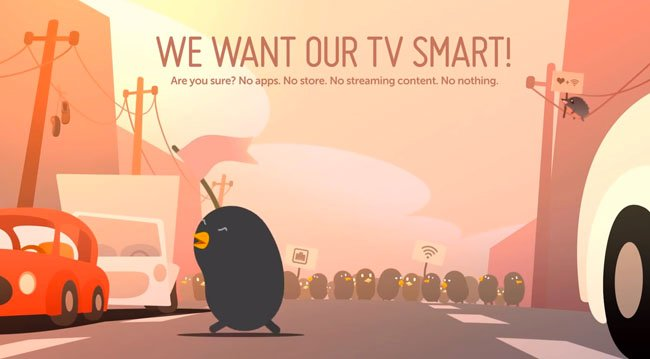
\includegraphics[width=0.7\textwidth]{lg_bean_bird_dialogue.jpg}
    \caption{Bean Bird demands internet\cite{damir_2014}.}
    \label{Bean_Bird}
\end{figure}
\newpage
\subsubsection{WebOS 6.0 2021}
In the early part of 2021, LG detailed and released samples of their WebOS 6.0 update, featuring a complete refresh of the interface and menu layouts. Most of the unique design elements that set WebOS apart from their competitors are gone and the resulting interface looks very similar to Google TV or Tizen.  
The response from both tech journalists and users is generally negative, citing the change to a content laden home screen cluttered with extraneous information and no options to customize the content listed. The launcher is gone and is replaced with a grid system similar to AppleTV. Since there are no TVs available with this version of the OS currently, a deeper analysis is not currently possible.
\begin{figure}[h]
    \centering
    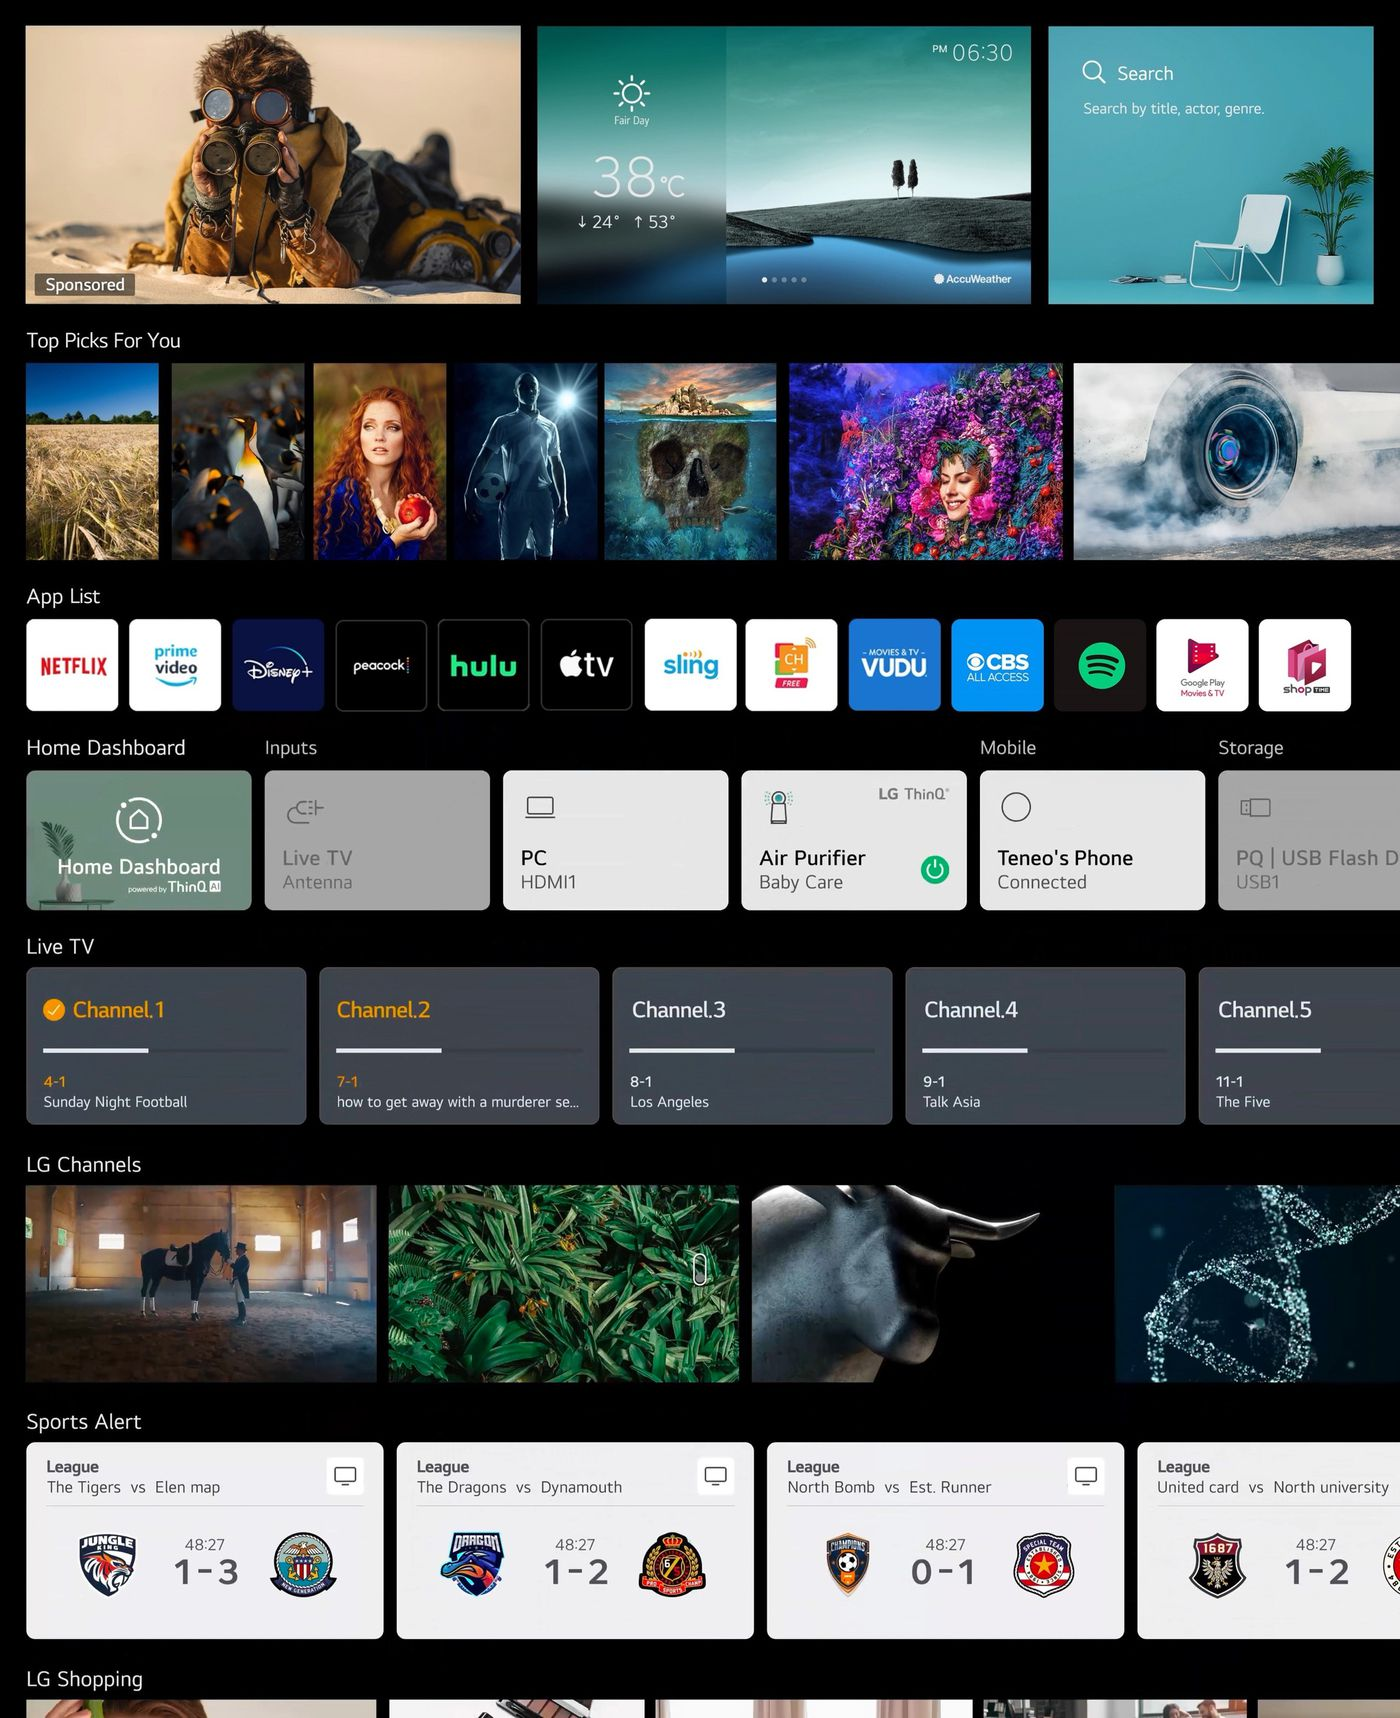
\includegraphics[width=0.7\textwidth]{LGwebos6.jpg}
    \caption{The unpopular 2021 webOS home screen}
\end{figure}
\subsection{Control Interfaces}
WebOS based smart TVs has a range of input options for users.  The "Magic" remote provided with the TV has motion sensors allowing it to be used as a pointing device, similar to the wiimote from Nintendo.  The motion tracking is smooth and responsive, and the cursor location can be reset by gently shaking the remote.  The remote also 
has a built in microphone, allowing users to search for content and issue commands.  ThinQ is the AI assistant built into WebOS, but newer versions also support Google Assistant and Alexa.  In addition, voice commands can be issued to smart speakers located in the same area, and a Bluetooth keyboard can be connected for easier text entry.  There is also a 
companion app for smartphones that can be used as a remote or to share content to the screen. 
\begin{figure}[h]
    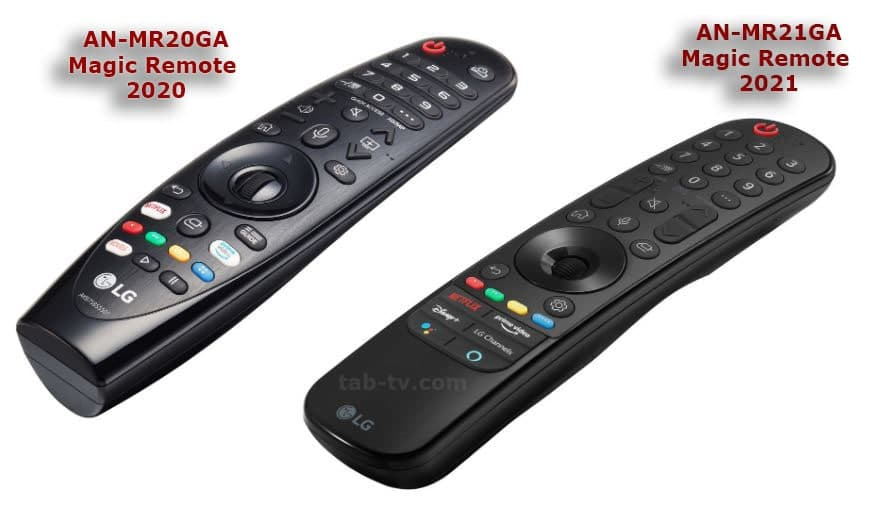
\includegraphics[width=\textwidth]{photo_2021-02-21_01-30-17.jpg}
    \caption{Comparison of 2020 and 2021 magic remote. The newer iteration has even more dedicated sponsor buttons.}
\end{figure}

The Magic Remote is simple and easy to use with minimal clutter.  The remote is curved and weighted more heavily towards the bottom of the remote, and small enough for people with a range of hand sizes to hold it and reach all the buttons.  The remote has motion tracking for the pointer functionality, allowing for easier text entry and maneuvering in the built-in web browser, as well as a 
four directional circular D-pad and a clickable scroll wheel.  The menus and launcher can be navigated with either the D-pad or the motion controls, but not all apps support pointer control.  The remote has dedicated buttons for opening the input sources, settings, and app launcher, as well as a microphone button.  The volume, channel buttons, and main navigation controls are positioned to be readily accessible to the user's thumb when held normally.  
Buttons are clearly labled and have different and logical tactile feelings, requiring less use of memory on the part of the user.  Later versions of the remote have sponsored service buttons, allowing for instant access to certain streaming services.  Each new iteration has added more of these buttons, leading to more clutter, especially for people that do not use those services.
There is also a row of multi\-use function buttons in bright primary colors.  These buttons can be used in applications and their function should be clearly listed.  The scroll wheel is located in the center of the D-pad and doubles as the select button.  The dedicated scroll function makes navigating large vertical lists much easier.
\subsection{User Feedback}
User feedback on the UI design was assessed based on user reviews on Amazon and Newegg.  Only medium to long reviews were considered, and only parts specifically about the UI or the input methods were used. Some of the issues highlighted in the user reviews may not be present in all versions of the OS. Privacy in particular seems to decrease in later versions of the OS.

Overall, the reviews of WebOS are positive, especially in tech journalism publications. 
WebOS received the top score in 2019 in a comparison between different smart TV and streaming device options for its ease of use and powerful voice assistant\cite{westover_2019}. The unobtrusive design of the app launcher and the bright color scheme are also notable mentions. User reviews are more varied, most people enjoy the design of the Magic remote, but some note difficulty learning all the features. Another negative issue mentioned in the reviews was illogical menu arrangement and 
video profiles overwriting previous settings\cite{nitromethane}.  All tracking options are enabled by default on newer versions as well, requiring users to navigate through the settings and disable them.  Some reviews noted that that process was not too difficult, however. Setup and app availability received positive reviews as well\cite{christy}.
\subsection{Areas for Improvement}
Overall, WebOS is one of the most approachable and enjoyable to use TV operating systems.  Menus are clear and unobtrusive, input methods are varied and meet multiple use cases, and the setup is streamlined and rewarding for the user through the use of a personable virtual agent. While the launcher and other content-related menus are straightforward and easy to use, the settings menus leave something to be desired.  The overall design is clean looking and easy to use, but picture settings are split across
different categories, and the included video profiles can overwrite other settings without warning.  A unified video settings panel and a default user profile would help address these issues. Requiring users to opt out of anti-privacy settings is also ethically challenging, especially with an interface otherwise designed to avoid users needing to search through menus.  The amount of data tracked by LG is extensive, including content viewed, voice data, ad data, and viewing data.  Disabling these features also
limit access to some features on the TV.  Better transparency and opt-in tracking would be more friendly to users. One final issue with the interface is a lack of consistent support for all input methods across applications, especially in older versions of the OS.  Some apps support point and click, while others only support D-pad entry. App developers are also inconsistent with their use of WebOS's built-in keyboard, opting to use their own design instead.  This lack of consistency in design standards can lead to 
user frustration when the input methods don't work as expected.  
\section{TizenOS}
TizenOS is Samsung's smart TV and IoT operating system. Similar to WebOS, Tizen is an open source OS based on Linux and is primarily used by Samsung watches, TVs, cars, and appliances. Tizen currently has the largest market share of Smart TVs as of 2020 at 12\% globally\cite{strategy_analytics_2020}.  Tizen's TV UI draws a lot of inspiration from WebOS.
\subsection{GUI}
The Tizen interface on TVs is called Eden UI. Similar to WebOS, Eden features an application launcher ribbon along the bottom half of the screen. Unlike WebOS, Eden's launcher allows apps to set custom icons and logos on the cards. This leads to a less consistent aesthetic overall, but may increase recognition based on branding. Applications are represented by small rectangular cards, and focused cards are expanded to make it obvious that they are selected.  They also have a small triangular shape towards the 
bottom of the card, similar to the selector on a dial.  When a card is in focus, a second panel containing suggested and recent content appears above the launcher ribbon. The information and quick access links in this panel vary in functionality, allowing the user to access their DVR and other set top box features if the box is properly connected. The preview panel requires app developers to support that functionality in their apps instead of generating something automatically, so some applications will not have the panel popup.
Menus for the channel list, channel guide, and most watched channels are all available directly from the launcher ribbon. On the far left end of the launcher are icons for keyword search, the input menu, and a panel containing recent and suggested apps.
\begin{figure}[h]
    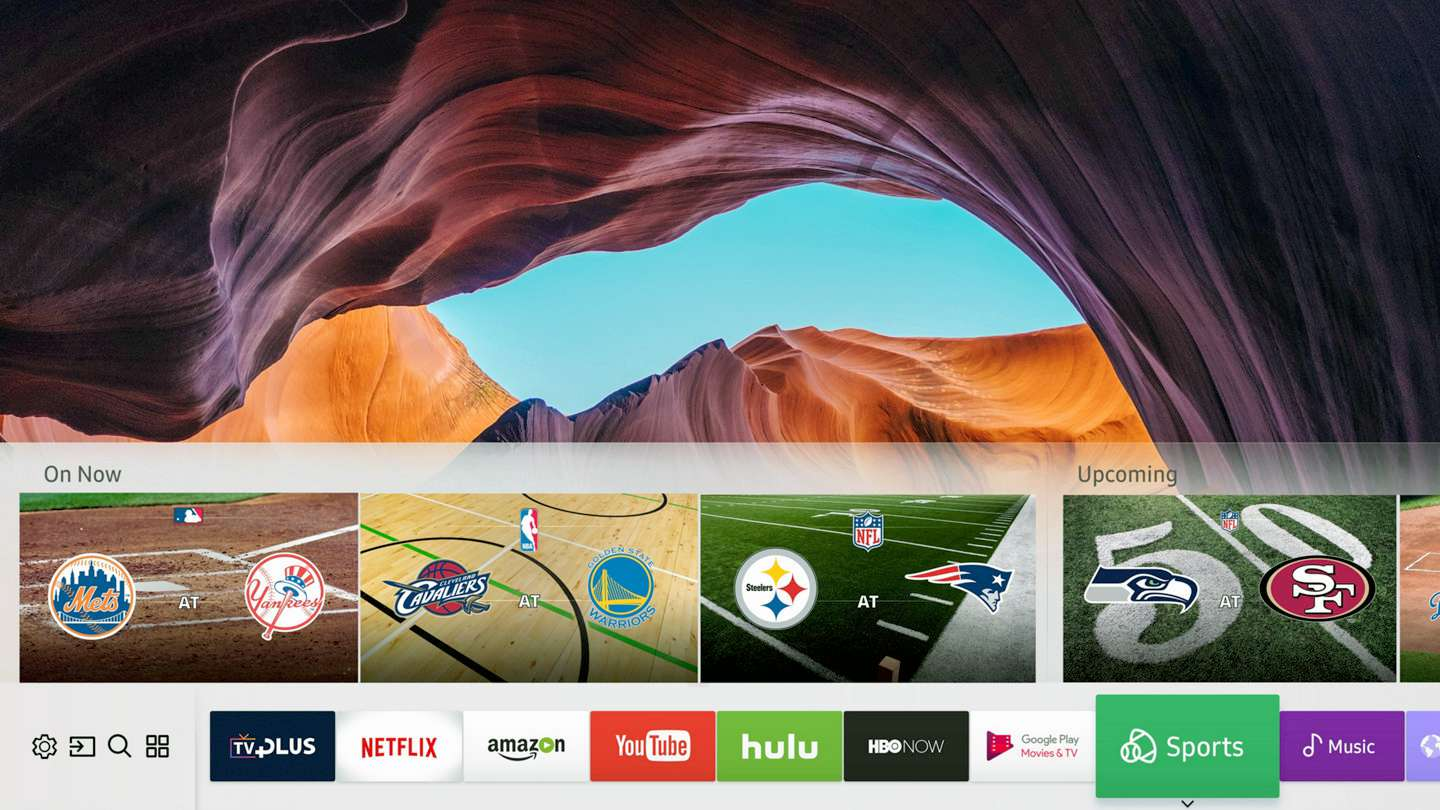
\includegraphics[width=0.9\textwidth]{samsung-tizen-2017-aaa-5a2c4d0e96f7d000373bfb76.jpg}
    \caption{The TizenOS App Launcher}
\end{figure}
\newpage
The overall aesthetic design of the Eden UI focuses heavily on semitransparent white and gray panels with mainly blue accent colors. Drop shadows give a sense of depth, and menu items shift in size and position as they are focused on. The Eden UI implementation of TizenOS shares many similarities of design with WebOS including smooth animation of most menu elements. Icon meanings are clear and range from minimalist to fairly detailed. Along with the input menu is a guide for connecting different devices to the TV including consoles and mobile devices.  
Given the large number of options for connecting devices, presenting users with an easily accessible and detailed manual is important for ease of use. 

Tizen also recognizes devices plugged into the HDMI ports and lists them by device name in the input menu, eliminating the struggle of remembering which input has which device.  This information is also used to automatically register devices on the smart remote.
There is also a quick settings panel located in the same area on the ribbon, allowing users to access and change the most common settings such as picture and audio. Users can cycle through video profiles, and there is a small arrow that indicates whether users can pull up a more granular menu for that specific setting.  Each quick setting icon also has a set of dots underneath indicating how many options there are to choose from.
In addition to the animations on cards and general menu features, the icons themselves are animated in some cases, communicating the change in settings in a noticeable but non-distracting way.  Overall, the Eden UI is a cleaner, more minimalist version of WebOS with less of a focus on bright, contrasting colors and without the whimsical animations. In particular, the layout and grouping of options in the settings menus are much more consistent.
\subsection{Control Interfaces}
The Samsung smart remote is the primary input device for the Tizen OS. The remote is designed to work as a universal remote for all relevant devices and accessories such as audio systems and set top boxes. The remote uses a very minimalist button layout.  There are no dedicated volume or channel arrow buttons, and no number pad.  Instead, there are just 10 buttons in total, including a D-pad navigation ring.  To enter numbers, the user needs to press the number button and then use the on-screen entry menu to make changes. Volume and channels are changed using small rocker buttons. 
Similar to the LG Magic remote, there is a dedicated voice command button, intended to be the primary method for entering text and searching for content.  THere is also a dedicated smart home control button for opening the built-in smart home hub. Unlike many other smart remotes, there are no buttons specifically dedicated to opening services like Netflix or Hulu. There are no motion controls, limiting navigation to directional inputs and voice commands.  There is a smartphone app that allows the use of a mobile device as a remote, however, and newer versions of Tizen support Amazon's Alexa, also usable
through the smart remote.  While the smart remote is simple and uncluttered, many of the affordances of more traditional remotes such as dedicated arrows for volume or easy number input with a number pad are lost.  This could be a particular issue for the visually impaired.  Another input option is a keyboard and mouse, either wired or over Bluetooth.
\begin{figure}
    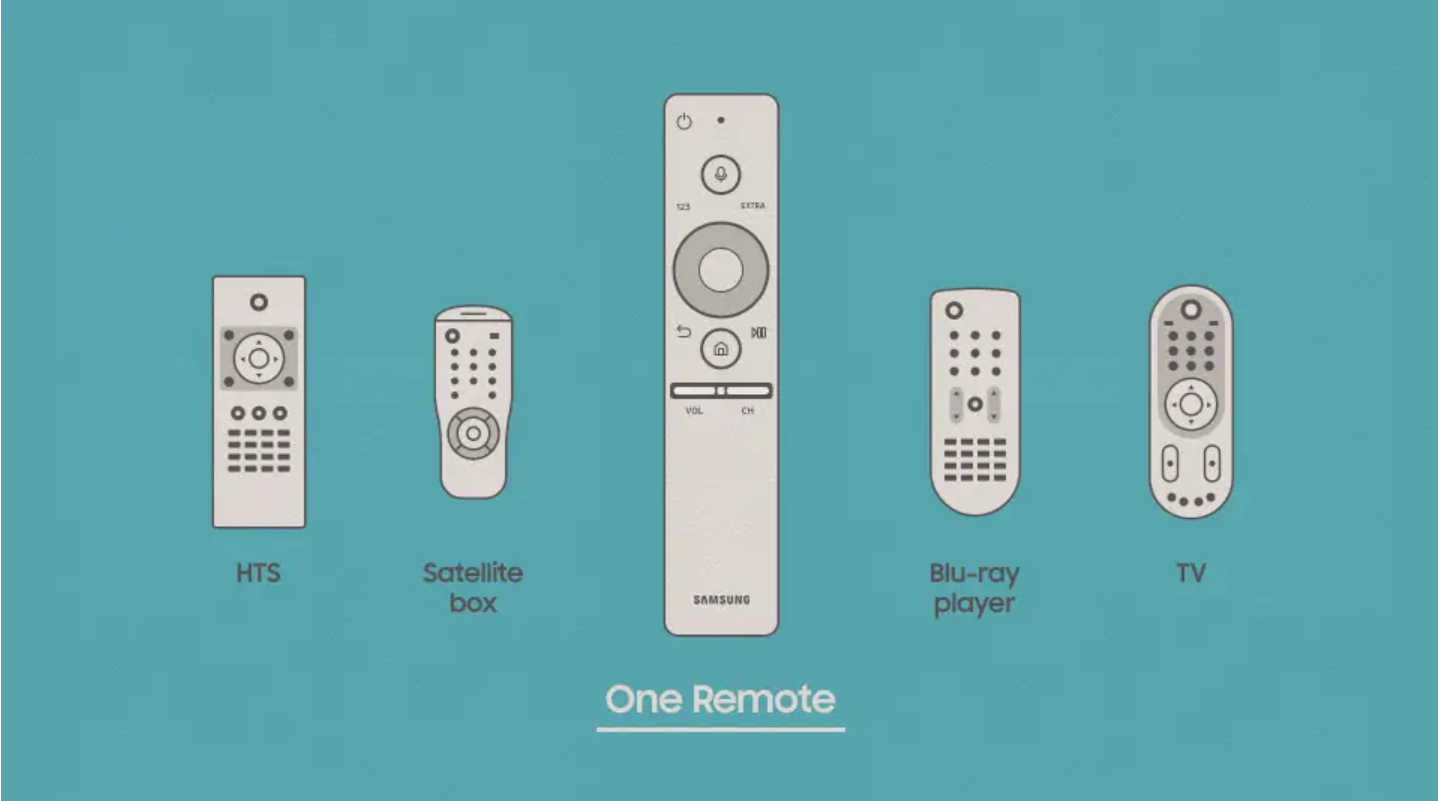
\includegraphics[width=\textwidth]{Screenshot 2021-04-24 110158.png}
    \caption{Samsung's Universal Remote}
\end{figure}
\subsection{User Feedback}
For the most part user reviews of Samsung smart TVs focus less on the smart features and more on the TV quality. Tizen is straightforward to use and has a well-developed app ecosystem, assuming the TV the OS is installed on has the necessary features. Unfortunately Samsung has moved in the direction of displaying ads on the UI home screen.  Sponsored apps are impossible to uninstall, leading to unnecessary bloat. The built in screen sharing functionality is also unreliable. The fundamental design of the Tizen OS is well liked, but the bloatware and obtrusive adware is greatly disliked by reviewers, and is hard to excuse on a \$1000+ TV.
The Samsung smart remote has mostly positive reviews.  The minimal button count and lack of sponsored buttons is considered a plus by most, but some reviewers noted that a full number pad would be preferable to the on-screen input, and that the volume rocker could be overly sensitive. The automatic registering of connected devices is a major selling point from an ease-of use perspective, however. 
\subsection{Areas for Improvement}
The most glaring problem with the UI design is Samsung's decision to target advertisements to users on the launcher menu\cite{smith_2019}.  An possible solution for the benefit of user interaction would be to allow users to disable advertisements, or to limit the visibility to intermittent periods. There is also a wide variety of additional media display options, including social media dashboards and info panels. All this extra information can detract from the TV watching experience and violate the principles of UI design for Smart TVs regarding the reduction of features unnecessary for the primary goal of consuming content.
The design of the Smart universal remote is effective and fairly simple to use, but could benefit from more traditional volume inputs and back lighting.
\section{tvOS}
tvOS is one of the most consistently well styled TV platforms, with a clearly articulated design philosophy and a thorough UI toolkit for developers.  Apple's tv platform has a low share of the U.S. market share at around 2\%, especially compared to Samsung, but they are fairly new to the streaming device market and are higher priced compared to Chromecasts or Roku products. The UI has a heavy focus on small details to make the presented content as interesting and immersive as possible, while the remote is simple in design yet flexible enough for menu navigation or use as a game controller. Apple's reputation for 
user-friendly interfaces is well represented.
\subsection{GUI}
tvOS's UI centers around a main home screen for grouping apps and content, with a grid-based layout. There is not a launcher bar for apps like Tizen or WebOS had, but at the top of the home screen there is a set of frequently used apps along with a large expanse of free space for app related imagery. Apple uses a focus based model for designing their tvOS UI, clearly yet unobtrusively indicating what tiles or items are selected on screen.  Rather than changing the colors or borders around items when the user has focused on that item, the tile will expand in size, appearing to grow larger compared to the rest of the tiles.  Enough padding surrounds each tile to allow for this expansion without the focused tile
overlapping with the surrounding tiles.  Shadows become more pronounced, giving a strong feeling that the content is closer to the user, and the text label for the tile is visible below the tile in a contrasting color.  This sense of closeness is consistently used to indicate which menus and other types of content are currently in focus. When a user focuses on a tile, they can gently shift the tile around using the remote's touch surface.  When the tile is moved this way, it appears to reflect the lighting in the menu, as well as displaying a subtle parallax effect.  Parallax is a major part of the tvOS design language and is used throughout the UI on icons, tiles, and other focusable toggles. Apple has clear standards for 
UI tile and button animations, including unfocused, focused, and highlighted. The highlighted state only shows for a moment, and is generally animated to show the focused item being pushed similar to a button, a helpful metaphor especially with a design language that discourages more common selection indicators such as border changes.  The drop shadow also changes, and the tile appears to be further from the user than the focused state, but still raised above the other tiles\cite{designing_for_apple_tv}.  
\begin{figure}
    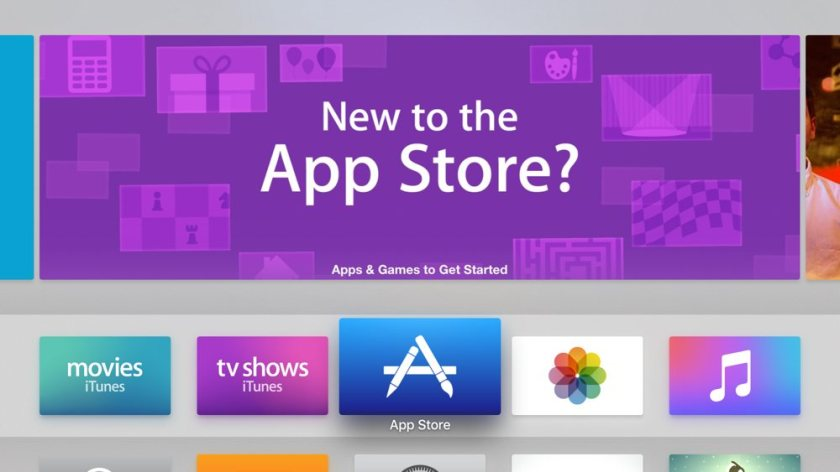
\includegraphics[width=\textwidth]{tvos_home_screen.jpg}
    \caption{tvOS home screen featuring focused tile.}
\end{figure}

Apps follow a consistent hierarchy of levels with increasing focus on content, and the menu button will always return the user one level higher in the application or general UI.  Whether 
the user is in a game or looking at movies in Apple TV+, clicking the menu button will bring the user to the previous page and eventually back to the homescreen.  This consistency gives the UI a very intuitive feel as it is impossible to get lost in menus.  There is a strong focus on immersion, so Apple maximizes the amount of screen space that can be filled with large images, removing clutter from the screensavers and reducing the amount of space for text when viewing content information screens, allowing for a large image to be shown in the background. tvOS's consistency and intuitiveness across contexts combined with satisfying animations and details on the heavily interacted parts of the UI makes Apple TV a generally positive user experience,
especially since the OS is consistently installed on hardware powerful enough to not face stutter or other performance issues. 
\subsection{Control Interfaces}
The primary method of controlling the Apple TV is the Siri remote, a small, thin rectangle with six buttons and a touch surface. The remote also features a built in microphone for controlling the TV using Siri, and a gyroscope and accelerometer for motion controls in video games. There are two dedicated volume buttons, a Siri button, a play/pause button, a menu button, and Home button. The menu button can be used to move one step up whatever menu hierarchy the user is currently in, giving users a consistent way to navigate out of parts of apps. The play button can be used to skip the info screens on tiles, allowing the user to instantly play content rather than viewing more information for their selection. The button can also be used as a functional button
in third party apps. The main navigation functions are performed using taps and gestures on the remote's touch surface. Lists of content can be quickly scrolled through by swiping, or advanced granularly with taps in a specific direction. Selections require firmly clicking the touch pad area, rather than tapping to prevent accidental activation. Tiles are also wiggled using the touch pad.  tvOS uses two different approaches for navigating groups of content, whether images in an app or tiles.  When there are multiple selectable items on the screen, swiping moves the viewport in the direction of the swipe, as if the menu is being dragged in the opposite direction to where the user is swiping. If there is only one item visible at a time, as in the case of looking at 
pictures in a photos app, then the traditional effect of dragging the content in the direction of the swipe occurs.  The unique way of navigating through multiple items by moving the focus of the screen is highly effective in the large format of a TV, reducing the amount the user needs to swipe.  

Unfortunately, the remote does have some usability issues.  The remote is very thin and light, and can easily slip between couch cushions or otherwise get lost. The remote is also one color, with black buttons on a black background, and there are no markings to indicate which parts of the touch pad are actually touch sensitive. The lack of a dedicated back button is also confusing to some users, as they don't realize the menu button serves that purpose.

tvOS can be controlled with voice commands from Siri, including switching apps, controlling videos, playing music, and getting information on listed content or other topics\cite{apple_support}. Apple TV can also be controlled via an iPhone or other Apple product over Airplay, allowing for casting of content and use of a virtual remote. HomePods and other Apple smart speakers can also be connected and used for audio output and control via Siri. Finally, Bluetooth game controllers can be connected and used for navigation as well as game play.
\begin{figure}[h]
    \centering
    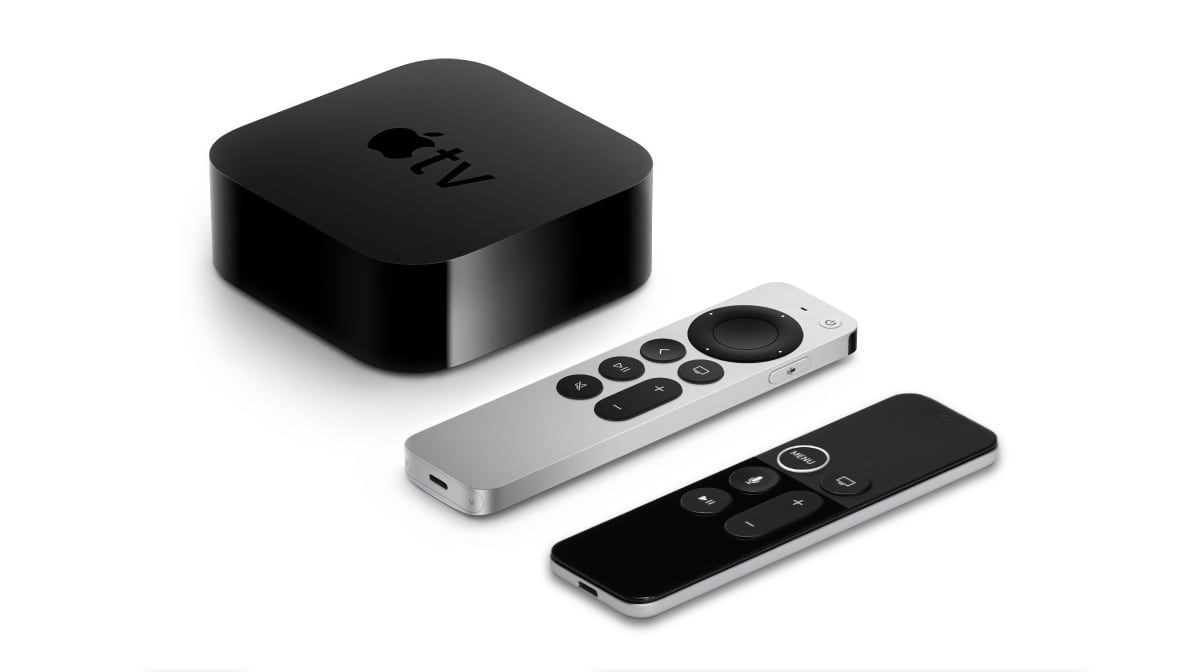
\includegraphics[width=0.8\textwidth]{appletvremote202117_small.jpg}
    \caption{Apple remote 2020 vs 2021}
\end{figure}

\subsubsection{2021 Siri Remote}
Announced on April 20th, the new Siri remote fixes some of the major issues with the previous version. The menu button has been replaced with a back button, and the remote is now white with black buttons.  The Siri button has been moved to the side and the touch area is clearly visible. A mute button and power button have been added as well, and the remote is larger and easier to keep track of. The touch pad also features a satisfying tactile dial that can be used for scrolling and other uses. Motion controls are no longer supported, however.
\subsection{User Feedback}
By far the most common complaint about the Apple TV is how hard to use the remote is. The touch pad has sensitivity issues and is the only navigational input aside from Siri, leading to a tedious setup process and difficulty navigating menus\cite{beergod}. Menus are also more complicated than earlier versions of Apple TV, so there is an unpleasant learning curve for some people. A lack of preloaded apps also forced users to navigate through the app store to install programs, making the initial setup process take more time.  The clean, consistent themeing and frictionless integration with other Apple products makes it a good choice for many people, regardless of some issues with the remote\cite{reader}.
\subsection{Areas for Improvement}
With the release of the 2021 Apple TV 4k, many of the issues with the older remote should be fixed but without access to the device or reviews, the level of improvement can only be speculated about. Apple's UI design standards are highly praised, and tvOS maintains those standards well. Apple's rigorous developer standards also maintain a higher level of UI consistency between the main UI and third party apps, reducing the memorization required. Simplifying some of the gesture usage for bringing up info panels and other functions could reduce some of the cognitive overload issues regarding menu complexity.
\section{Conclusion}
User experience and interface design has come a long way since the early days of smart TVs. TVs and streaming boxes are equipped with more powerful hardware, allowing for the use of animations and effects throughout with very little performance issues, and the overarching goal of serving content to the user with minimal required interaction is well accounted for through the use of virtual assistants such as Siri and Alexa, as well as a variety of smart remotes. 

A more worrying trend is the overabundance of bloat, data harvesting and targeted ads, especially on the home screen or launcher bar in the case of TizenOS. Smart TVs can be an expensive purchase and are generally long-term purchases with low turnover. Placing targeted ads and preventing the removal of sponsored apps on 
such an expensive purchase is very negative for the user and seems to be gaining more traction with TV brands.  While the interface and input methods range from sometimes confusing to fun and engaging, increased privacy and security concerns detract from the overall design, especially when the option to disable those features is hidden or unavailable.
\newpage
\printbibliography
\end{document}